\chapter{Discussion of results} \label{cha:Discussion-of-results}

\subsection{Gravitational assists}

Due to the low thrust of spacecraft \BW, it is expected that a substantial part of the orbit raising will be achieved by exploiting gravitational assists from the Moon. This technique has been well studied, although previous higher-thrust missions did not find it efficient to attempt more than one or two lunar resonances. \textcite{Kemble2006} explains that \enquote{It is possible to utilise lunar gravity to assist in the orbit raising prior to lunar encounter. This takes the form of a \emph{gravitational pumping} effect if the correct phase with respect to the Moon can be established}. He goes on to quantify that \enquote{A typical $\Delta V$ saving of 800~ms$^{-1}$ is obtained by use of lunar gravity assist}. Due to the extended duration of \BW's transit, more lunar resonances should be possible than in a \enquote{typical} scenario, so this should reduce the required delta-v for \BW's ascent from GTO to lunar orbit from 4.1~kms$^{-1}$ to less than 3.3~kms$^{-1}$.

Because lunar gravitational assists provide delta-v without fuel expenditure, they should be implicitly accounted for during optimisation. Preliminary results have already shown this to be the case, as seen in \autoref{fig:Lunar_resonance}. From an initial orbit of 180,000~km (semi-cis-lunar, representing the later stages of the transfer to highlight the lunar assist) the spacecraft takes two orbits to align its phase with the Moon, then receives a very apparent boost purely from the Moon's gravity.

\subsection{Oberth effect}

Regarding the thrust profile, it is well known that thrusting at particular points in the orbit are more efficient than others. \textcite{Kemble2006} once again explains, \enquote{Insertion of coast arcs allows the apogee raising input to be concentrated closer to perigee and hence increase the efficiency of the transfer (in terms of $\Delta V$ required)}. The reason for concentrating thrust near the perigee is known as the Oberth effect: over a period of thrusting, the specific orbital energy gained per unit delta-v exerted is equal to the instantaneous speed \parencite{Oberth1923}. Therefore thrusting is more efficient at high speed, which occurs at periapsis.
 
The resultant effect on the trajectory is that when variable thrust is implemented, the majority of the thrusting should occur near perigee; there should be an inverse relationship between thrust magnitude and orbital radius. 

\begin{figure}
\centering
%\input{Images/thrust-vs-time.jpg}
\caption{Thrust profile during orbit raising.}
\label{fig:Thrust_profile}
\end{figure}

Continuous thrust (tangential to the orbital radius) leads to circular trajectories because an eccentric starting trajectory spends more time at apoapsis than periapsis; hence more thrusting occurs at apoapsis than periapsis. As demonstrated by a Hohmann transfer, thrusting at apoapsis circularises the orbit.

The cycling observed in the figure is due to the elliptical orbit; at apogee and perigee the spacecraft is travelling perpendicularly to its position vector, resulting in a pitch angle of zero. As it travels towards the Earth, it has negative pitch angle, and positive pitch as it travels away again.
 
\begin{figure}
\centering
%\input{Images/pitch-vs-time.jpg}
\caption{Pitch angle during the orbit raising.}
\label{fig:BW1-Pitch}
\end{figure}

As observed in \autoref{fig:Thrust_profile} the thrust of \BW\ is almost constant throughout this simplified scenario. Consequently the traditional parameter for aircraft performance, thrust-to-weight ratio, seen in \autoref{fig:BW1-T/W-ratio}, is dominated by the changing effective weight, as the spacecraft moves closer to the Earth and then away again.

\begin{figure}
\centering
%\input{Images/thrust-to-weight-and-radius-vs-time.jpg}
\caption{\BW\ T/W ratio compared to radial position during the orbit raising. Plot exported from ASTOS.}
\label{fig:BW1-T/W-ratio}
\end{figure}

A spacecraft orbiting the Moon (in the same direction as the Moon orbits the Earth) undergoes a period of low velocity relative to the Earth every time it is on the Earthward side of the Moon. A spacecraft orbiting the Earth in a highly elliptical orbit undergoes a period of low velocity relative to the Earth when it reaches apoapsis, which is conveniently also the furthest point from the Earth, as shown in \autoref{fig:Apoapsis-and-periapsis}. Therefore the trajectory is expected to deliver the spacecraft at apoapsis to a \enquote{stationary point} in the intended lunar orbit, such that the Moon's gravity will then pull it into a steady lunar orbit, avoiding the need for a high-thrust capture maneuvre.

\begin{figure}
\centering
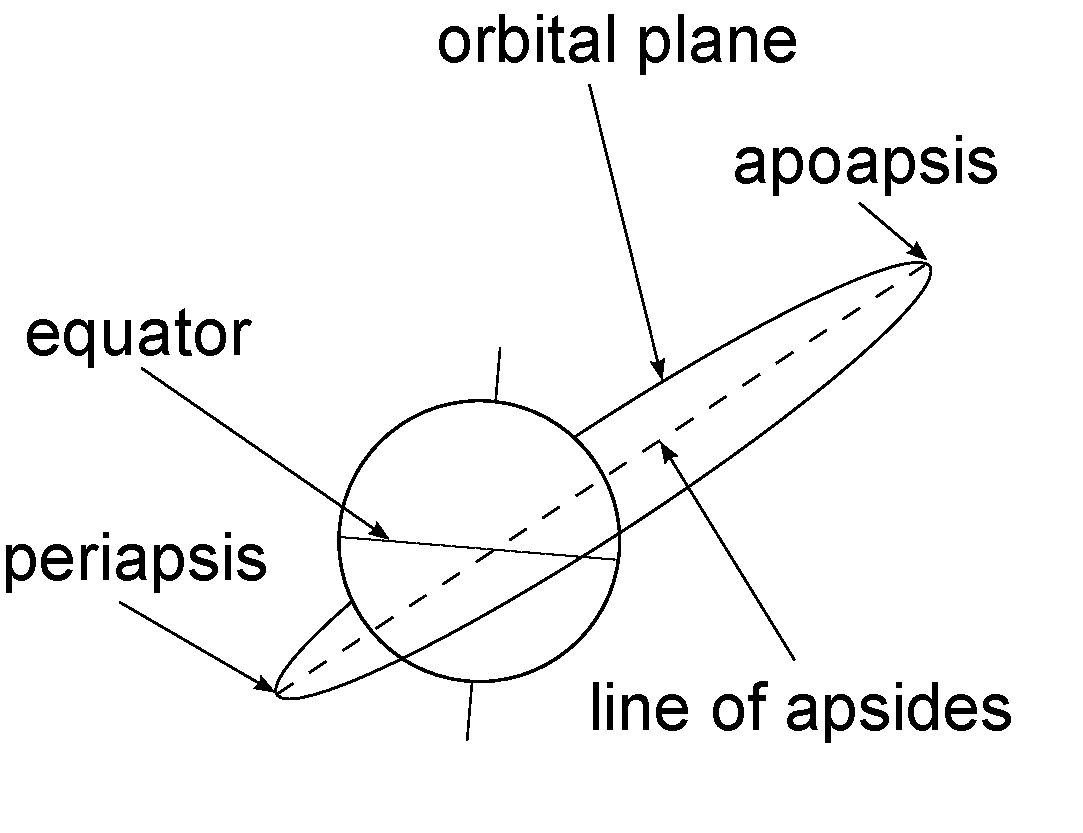
\includegraphics[scale=0.4]{Images/apsides.pdf}
\caption{Apoapsis and periapsis.}
\label{fig:Apoapsis-and-periapsis}
\end{figure}

To maximise the gravitational effect of the Moon on the spacecraft, it should be phase-locked with respect to the Moon's orbit. However, this would require constantly adjusting the orbital line of apsides, which is a high delta-v maneuvre. Gravitational resonance is generally exploited by pointing the apoapsis towards the Moon's ascending node (to remove any dependence on inclination) and adjust the orbital period to resonate with the Moon (that is, the spacecraft completes two orbits to every lunar orbit, or three orbits to every lunar orbit, or five orbits to every two lunar orbits, etcetera). However, based on the unique thrusting constraints of \BW, an alternative optimal scenario may be to maintain the fastest part of the orbit (periapsis) within the Earth's shadow (eclipse), to minimise the amount of time that the craft cannot charge its batteries. In this scenario the spacecraft should also thrust as it passes through the eclipse since it cannot recharge during this time, and thrusting will help it to escape the eclipse as quickly as possible. It will also be interesting to see whether it is optimal to correct inclination, apoapsis or eccentricity first, or whether the optimal solution adjusts all of these parameters simultaneously.
 
% It is well known how to most efficiently control various aspects of an orbit by thrusting at fortuitous times: increasing apoapsis efficiently by thrusting near periapsis, inclination by thrusting out of the orbital plane at apoapsis, and so forth, as anticipated by \textcite{Dachwald2007} in their discussion of optimisation results. \citet{Gao2008} outlines a convenient mathematical model to generate continuous, smooth parameters describing thrust steering, which can easily be used in an optimisation engine.

%\textcite{Edelbaum1964} gives an outline of some optimal low-thrust maneouvres (a, e, plane changes)
% arg of periapsis most efficiently changed at low eccentricity, inclination at high eccentricity, RAAN constant, a at periapsis.
 
% quantify stochastic & deterministic inputs, robustness

\section{Reduced complexity optimisation}

In order to get an initial idea of the optimal thrust profile, a reduced complexity trajectory was modelled. This was simply implemented by turning off secondary and tertiary perturbations, and optimising over a coarser mesh. 


\begin{figure}
\centering
\def\svgwidth{\figurewidth}
\input{Images/Ascent2/figure1.pdf_tex}
\caption{Reduced complexity ascent trajectory in ECI frame.}
\label{fig:Ascent2-3D}
\end{figure}

\begin{figure}
\centering
\def\svgwidth{\figurewidth}
\input{Images/Ascent2/figure10.pdf_tex}
\caption{Satellite's distance from Earth and Moon during reduced complexity ascent.}
\label{fig:Ascent2-dist}
\end{figure}

\begin{figure}
\centering
\def\svgwidth{\figurewidth}
\input{Images/Ascent2/figure7.pdf_tex}
\caption{Keplerian elements of satellite within ECI frame during reduced complexity ascent phase.}
\label{fig:Ascent2-kep}
\end{figure}

\begin{figure}
\centering
\def\svgwidth{\figurewidth}
\input{Images/Ascent2/figure9.pdf_tex}
\caption{Equinoctial elements of satellite within ECI frame during reduced complexity ascent phase.}
\label{fig:Ascent2-mee}
\end{figure}

\begin{figure}
\centering
\def\svgwidth{\figurewidth}
\input{Images/Ascent2/figure11.pdf_tex}
\caption{Orbital energy of the satellite relative to Earth and Moon during reduced complexity ascent phase.}
\label{fig:Ascent2-orbeng}
\end{figure}

\begin{figure}
\centering
\def\svgwidth{\figurewidth}
\input{Images/Ascent2/figure4.pdf_tex}
\caption{Perturbing accelerations acting on spacecraft during reduced complexity ascent phase.}
\label{fig:Ascent2-pert}
\end{figure}

\begin{figure}
\centering
\def\svgwidth{\figurewidth}
\input{Images/Ascent2/figure5.pdf_tex}
\caption{Perturbing accelerations acting on spacecraft during reduced complexity ascent phase.}
\label{fig:Ascent2-pert2}
\end{figure}

oscillations between ur and utheta - similar result to that discovered by \textcite{Betts2003}
interesting... main objective of this study... discover an optimal thrust profile given power constraints. Thrust when near periapsis.

\begin{figure}
\centering
\def\svgwidth{\figurewidth}
\input{Images/Ascent2/figure2.pdf_tex}
\caption{Direction of thrust vector during reduced complexity ascent phase.}
\label{fig:Ascent2-thrust}
\end{figure}

\begin{figure}
\centering
\def\svgwidth{\figurewidth}
\input{Images/Ascent2/figure3.pdf_tex}
\caption{Magnitude of thrust vector during reduced complexity ascent phase.}
\label{fig:Ascent2-thrustM}
\end{figure}

% Mass (6) 
% Delta-v (8)
% Phase (12)
% kep LCI (13)
% kep SEL (14)
% 3D SEL (15)


Following the reduced complexity ascent, optimisation was attempted for a reduced complexity cruise phase. However, due to the long duration of this phase and the limited computer resources available, the optimisation did not reach an optimal solution in the time available. This exercise did highlight other problems with the procedure, in particular determining a lunar capture. Due to the lunar orbit being very close escape energy relative to the Earth (only $5\times10^5 m^2s^{-2}$), the vast majority of simulations resulted in the spacecraft escaping the Earth's sphere of influence by gaining a gravitational assist from the Moon. This caused severe computational errors due to the anomaly ceasing to increase after escape. Another common failure scenario involved weak capture by the Moon, that is, after one or two orbits around the Moon the spacecraft would then be recaptured by the Earth. Due to the way the system was modelled, this once again caused computational errors: if the spacecraft is in orbit around the Moon in a Earth-centric frame, the anomaly is not guaranteed to be always increasing; the same applies for a spacecraft in Earth orbit during a lunar-centric frame.

Determining conditions for strong lunar capture proved difficult and unreliable. Consequently it was decided to simulate the transfer backwards, from lunar orbit to Earth orbit, using an industry standard tool called Satellite Tool Kit (STK) \parencite{STK}. Backwards propagation has been used by many previous authors, such as \textcite{Author}. The main advantage to this approach is that any ascent from lunar orbit must necessarily pass through Earth orbit; whereas the reverse does not apply. Furthermore, with the Moon in a 19\degrees\ inclined orbit about the Earth, any ascent from the Moon will end up in approximately the same plane as the parking orbit after launch, thus implicitly accounting for the plane changes required to achieve the target lunar orbit.

\clearpage

\section{STK modelling}

images from STK
continuous
not optimised
very limited number of optimisation parameters available; cannot even perform 2pbvp for continual thrust
therefore cannot target specific orbit, such as correct inclination and eccentricity of GTO
solves problem of lunar capture, but further work required (by GESOP) to complete feasible end-to-end orbit even before any optimisation takes place

\section{Ascent} 
The ascent phase was modelled in GESOP subject to the initial boundary conditions outlined in \autoref{tab:Phase-2-constraints} and final boundary conditions outlined in \autoref{tab:Phase-2-3-constraints}. An initial guess was taken for the thrust profile perpendicular to the orbital radius at all times throughout ascent, in order to raise the periapsis as quickly as possible beyond the van Allen belts.

The initial guesses for time and mass were taken from the STK simulation. Continuity conditions were imposed to connect the end conditions of this phase to the starting conditions of the cruise phase. This implementation of continuity is not ideal as it enforces an arbitrary position and velocity at the phase transitions, thus reducing the flexibility during optimisation. Ideally the phases would be optimised together, enforcing continuity between phases but not specifying what those conditions are. However this was not possible due to computational complexity, and remains an improvement for the future, perhaps exploiting parallel processing and supercomputer hardware.

Given the arbitrary nature of these continuity conditions, they were used for the initial guess but not enforced during optimisation. As the actual parameters moved away from their initial values during the optimisation, discontinuities emerged in the trajectory. This was permitted for a number of reasons. Firstly, the launch conditions are not known, so the procedure used in this optimisation is more important than the actual result. Secondly, the phase transitions still occur at very similar orbits, thus the variation in orbital energy was very small. In other words, the main difference between the orbits was simply timing, and at any of the phase transitions the spacecraft can sit in a parking orbit until the correct alignment occurs. Finally, due to the computational limitation of optimising each phase independently, any small change would then require all other phases to be recalculated. Treating each separately, with an implicit parking orbit in between, allows these small changes without any significant effect to the remaining phases.

\autoref{fig:Ascent-3D} shows the 3-dimensional trajectory that resulted from the ascent phase. This optimisation was able to reach a feasible solution in the computational time available, but was not allowed to continue on to find an optimal solution. Consequently the ascending orbit does not show the Oberth effect to such effect as in the reduced complexity optimisation.

\begin{figure}
\centering
\def\svgwidth{\figurewidth}
\input{Images/Ascent/figure1.pdf_tex}
\caption{Ascent trajectory in ECI frame.}
\label{fig:Ascent-3D}
\end{figure}

\autoref{fig:Ascent-dist} shows the distance of the spacecraft from the Earth and Moon throughout the phase. The oscillations about the Earth are seen to slowly increase in duration and altitude, as you would expect for a slowly ascending orbit. The spacecraft's apoapsis (furthest point from the Earth) occurs with approximately the same angle as the Moon's periapsis (closest point to Earth). This is an optimal scenario, as it leads to much greater gravitational assistance earlier on in the transfer, but is unfortunately not a scenario that can be planned for, as the initial argument of periapsis is defined by the launch. The optimisation is able to imiplicitly adjust the argument of periapsis during the transfer by controlling the thrust angle, but this technique requires a lot of delta-v and therefore can only compensate for a few degrees.

\begin{figure}
\centering
\def\svgwidth{\figurewidth}
\input{Images/Ascent/figure10.pdf_tex}
\caption{Satellite's distance from Earth and Moon during ascent phase.}
\label{fig:Ascent-dist}
\end{figure}

The orbital energy of the spacecraft relative to the two bodies shown in \autoref{fig:Ascent-orbeng} does not reveal much during this phase, except that the spacecraft is slowly ascending from, although still very much captured within, Earth's gravitational field. The orbital energy with respect to the Moon fluctuates wildly as the spacecraft orbits Earth, as the gravitational potential remains relatively constant but the craft's velocity vector rotates towards the Moon and then away again. It is interesting that at times even from the GTO parking orbit, the spacecraft is very close to lunar capture ($\epsilon_m\approx0$).

\begin{figure}
\centering
\def\svgwidth{\figurewidth}
\input{Images/Ascent/figure11.pdf_tex}
\caption{Orbital energy of the satellite relative to Earth and Moon during ascent phase.}
\label{fig:Ascent-orbeng}
\end{figure}

The thrust profile calculated by the optimisation is shown in \autoref{fig:Ascent-thrust}, along with the corresponding thrust magnitude in \autoref{fig:Ascent-thrustM}. While the scale of these results seems trivial, they are indicative of the direction the optimisation was pushing the solution, and suggest that the reduced complexity results form a good approximation. 

\begin{figure}
\centering
\def\svgwidth{\figurewidth}
\input{Images/Ascent/figure2.pdf_tex}
\caption{Direction of thrust vector during ascent phase.}
\label{fig:Ascent-thrust}
\end{figure}

\begin{figure}
\centering
\def\svgwidth{\figurewidth}
\input{Images/Ascent/figure3.pdf_tex}
\caption{Magnitude of thrust vector during ascent phase.}
\label{fig:Ascent-thrustM}
\end{figure}

\autoref{fig:Ascent-mee} shows the changing equinoctial elements of the orbit throughout the transfer, accompanied by the rather more intuitive keplerian elements in \autoref{fig:Ascent-kep}. Unsurprisingly, the semimajor axis $a$ and the semilatus rectum $p$ grow smoothly throughout the transfer, and their rate of growth increases as the spacecraft gets further from Earth's gravity well. The spacecraft's eccentricity $e$ slowly decreases as the continual tangential thrust raises the perigee faster than the apogee, but again, this is exactly as required during this phase.

\begin{figure}
\centering
\def\svgwidth{\figurewidth}
\input{Images/Ascent/figure9.pdf_tex}
\caption{Equinoctial elements of satellite within ECI frame during ascent phase.}
\label{fig:Ascent-mee}
\end{figure}

\begin{figure}
\centering
\def\svgwidth{\figurewidth}
\input{Images/Ascent/figure7.pdf_tex}
\caption{Keplerian elements of satellite within ECI frame during ascent phase.}
\label{fig:Ascent-kep}
\end{figure}

The stronger forces acting on the spacecraft during the ascent phase are shown in \autoref{fig:Ascent-pert}, and the weaker forces in \autoref{fig:Ascent-pert2}. It is immediately apparent that only the Earth's oblateness plays a significant role in defining the spacecraft trajectory from such a low orbit. However, as outlined in \autoref{sub:Oblateness} this only affects the argument of periapsis and right ascension of the ascending node, and therefore cannot be exploited to raise the orbit faster. As outlined above, adjusting the argument of periapsis may assist with lining up gravitational assists from the Moon later in the transfer, but due to the limitation of modelling phases separately this assist could not be incorporated. Consequently, the thrust profile was optimised purely for a fast ascent. Interestingly, the optimiser did adjust the trajectory starting date from the initial guess derived from STK, which has the effect of adjusting the phase between the spacecraft and the Moon. This shows that even the relatively weak lunar gravity present during this phase may still be exploited. The orders of magnitude between the forces shown in \autoref{fig:Ascent-pert} and the gravitational forces due to Jupiter, Venus and Mars in \autoref{fig:Ascent-pert2} highlight the reason why so many earlier studies neglect these forces. 

\begin{figure}
\centering
\def\svgwidth{\figurewidth}
\input{Images/Ascent/figure4.pdf_tex}
\caption{Perturbing accelerations acting on spacecraft during ascent phase.}
\label{fig:Ascent-pert}
\end{figure}

\begin{figure}
\centering
\def\svgwidth{\figurewidth}
\input{Images/Ascent/figure5.pdf_tex}
\caption{Perturbing accelerations acting on spacecraft during ascent phase.}
\label{fig:Ascent-pert2}
\end{figure}

The practically constant thrust results in a linear fuel consumption. Consequently this simulation suggested approximately 60~kg worth of ammonia would be required for the ascent phase. %compare to initial guess?

%\begin{figure}
%\centering
%\def\svgwidth{\figurewidth}
%\input{Images/Ascent/figure6.pdf_tex}
%\caption{Mass of spacecraft during ascent phase.}
%\label{fig:Ascent-mass}
%\end{figure}

% Mass (figure6)
% DeltaV (figure8)
% Phase (figure12)
% LCI kep (figure13)
% LCI 3D (figure14)
% SEL 3D (figure15)
% Energy (figure16)

\clearpage

\section{Cruise}
The initial guess for the cruise phase was also taken from the STK simulation, and subjected to boundary conditions as outlined in \autoref{sub:BVP}.
Multiple different initial guesses based on power - leading to lunar capture
optimising cruise phase forwards to given termination condition (SOI) causes numerical errors (gets pulled into lunar orbit and so L (ECI) is no longer independent, or gets thrown into escape trajectory and so L (ECI) no longer increases, or ...).
tried backward propagating from final orbit, but thrusting tangentially does not change inclination so it is difficult to achieve the nearly polar orbit required.
found that, due to the similar launch inclination coupled with the slow ascent leading to many lunar assists, almost any launch will end up near the Moon. The problem thus becomes ensuring lunar capture, rather than a lunar slingshot into an Earth-escape trajectory. This was achieved by modelling the scenario in STK, assigning arbitrary values for $\omega$ and $\Omega$, and then using STK's BVP solver to establish a feasible initial guess for the optimiser. 
Also, very difficult to achieve polar lunar orbit with forwards propagation. Backwards propagation from lunar orbit will ascend in polar orbit, until lunar escape velocity achieved. Provided it escapes in the right direction (and doesn't achieve Earth escape velocity) it goes into high Earth orbit near lunar inclination - which is relatively near to launch inclination. Try backwards propagation for the whole transfer?
circular orbit - rendezvous with moon can't really be scheduled, it will happen inevitably. can schedule effect of rendezvous perhaps? change inclination/eccentricity etc?

\begin{figure}
\centering
\def\svgwidth{\figurewidth}
\input{Images/Cruise/figure1.pdf_tex}
\caption{Cruise trajectory in ECI frame.}
\label{fig:Cruise-3D}
\end{figure}

\begin{figure}
\centering
\def\svgwidth{\figurewidth}
\input{Images/Cruise/figure10.pdf_tex}
\caption{Satellite's distance from Earth and Moon during cruise phase.}
\label{fig:Cruise-dist}
\end{figure}

\begin{figure}
\centering
\def\svgwidth{\figurewidth}
\input{Images/Cruise/figure11.pdf_tex}
\caption{Orbital energy of the satellite relative to Earth and Moon during cruise phase.}
\label{fig:Cruise-orbeng}
\end{figure}

Not optimised, so unitary thrust magnitude.

\begin{figure}
\centering
\def\svgwidth{\figurewidth}
\input{Images/Cruise/figure2.pdf_tex}
\caption{Direction of thrust vector during cruise phase.}
\label{fig:Cruise-thrust}
\end{figure}

\begin{figure}
\centering
\def\svgwidth{\figurewidth}
\input{Images/Cruise/figure7.pdf_tex}
\caption{Keplerian elements of satellite within ECI frame during cruise phase.}
\label{fig:Cruise-kep}
\end{figure}

\begin{figure}
\centering
\def\svgwidth{\figurewidth}
\input{Images/Cruise/figure9.pdf_tex}
\caption{Equinoctial elements of satellite within ECI frame during cruise phase.}
\label{fig:Cruise-mee}
\end{figure}


Thrust slowly increasing as mass drops due to fuel use.

\begin{figure}
\centering
\def\svgwidth{\figurewidth}
\input{Images/Cruise/figure4.pdf_tex}
\caption{Perturbing accelerations acting on spacecraft during cruise phase.}
\label{fig:Cruise-pert}
\end{figure}

\begin{figure}
\centering
\def\svgwidth{\figurewidth}
\input{Images/Cruise/figure5.pdf_tex}
\caption{Perturbing accelerations acting on spacecraft during cruise phase.}
\label{fig:Cruise-pert2}
\end{figure}

% Thrust magnitude (figure3)
% Mass (figure6)
% DeltaV (figure8)
% Phase (figure12)
% LCI kep (figure13)
% LCI 3D (figure14)
% SEL 3D (figure15)
% Energy (figure16)

\clearpage 

\section{Propagate}
Initial guess, simulation, optimisation

\begin{figure}
\centering
\def\svgwidth{\figurewidth}
\input{Images/Propagate/figure1.pdf_tex}
\caption{Propagate trajectory in ECI frame.}
\label{fig:Propagate-3D}
\end{figure}

\begin{figure}
\centering
\def\svgwidth{\figurewidth}
\input{Images/Propagate/figure14.pdf_tex}
\caption{Propagate trajectory in LCI frame.}
\label{fig:Propagate-3D-lci}
\end{figure}

\begin{figure}
\centering
\def\svgwidth{\figurewidth}
\input{Images/Propagate/figure15.pdf_tex}
\caption{Propagate trajectory in SEL frame.}
\label{fig:Propagate-3D-sel}
\end{figure}

\begin{figure}
\centering
\def\svgwidth{\figurewidth}
\input{Images/Propagate/figure10.pdf_tex}
\caption{Satellite's distance from Earth and Moon during propagate phase.}
\label{fig:Propagate-dist}
\end{figure}

\begin{figure}
\centering
\def\svgwidth{\figurewidth}
\input{Images/Propagate/figure11.pdf_tex}
\caption{Orbital energy of the satellite relative to Earth and Moon during propagate phase.}
\label{fig:Propagate-orbeng}
\end{figure}

\begin{figure}
\centering
\def\svgwidth{\figurewidth}
\input{Images/Propagate/figure7.pdf_tex}
\caption{Keplerian elements of satellite within ECI frame during propagate phase.}
\label{fig:Propagate-kep}
\end{figure}

\begin{figure}
\centering
\def\svgwidth{\figurewidth}
\input{Images/Propagate/figure13.pdf_tex}
\caption{Keplerian elements of satellite within LCI frame during propagate phase.}
\label{fig:Propagate-kep-lci}
\end{figure}

\begin{figure}
\centering
\def\svgwidth{\figurewidth}
\input{Images/Propagate/figure9.pdf_tex}
\caption{Equinoctial elements of satellite within ECI frame during propagate phase.}
\label{fig:Propagate-mee}
\end{figure}


\begin{figure}
\centering
\def\svgwidth{\figurewidth}
\input{Images/Propagate/figure4.pdf_tex}
\caption{Perturbing accelerations acting on spacecraft during propagate phase.}
\label{fig:Propagate-pert}
\end{figure}

\begin{figure}
\centering
\def\svgwidth{\figurewidth}
\input{Images/Propagate/figure5.pdf_tex}
\caption{Perturbing accelerations acting on spacecraft during propagate phase.}
\label{fig:Propagate-pert2}
\end{figure}

\begin{figure}
\centering
\def\svgwidth{\figurewidth}
\input{Images/Propagate/figure12.pdf_tex}
\caption{Angle between spacecraft and Moon during propagate phase.}
\label{fig:Propagate-phase}
\end{figure}

% Thrust direction (figure2)
% Thrust magnitude (figure3)
% Mass (figure6)
% DeltaV (figure8)
% Energy (figure16)

\clearpage

\section{Capture}
Initial guess, simulation, optimisation
Increase phase duration until it gets close to escape.
Adjust starting date until point where difference between satellite phase and lunar phase changes direction (i.e. satellite is near the same orbit as the moon) is close to 0\degrees.

\begin{figure}
\centering
\def\svgwidth{\figurewidth}
\input{Images/Capture/figure1.pdf_tex}
\caption{Capture trajectory in ECI frame.}
\label{fig:Capture-3D}
\end{figure}

\begin{figure}
\centering
\def\svgwidth{\figurewidth}
\input{Images/Capture/figure14.pdf_tex}
\caption{Capture trajectory in LCI frame.}
\label{fig:Capture-3D-eci}
\end{figure}

\begin{figure}
\centering
\def\svgwidth{\figurewidth}
\input{Images/Capture/figure15.pdf_tex}
\caption{Capture trajectory in SEL frame viewed from Moon's pole.}
\label{fig:Capture-3D-sel-above}
\end{figure}

%\begin{figure}
%\centering
%\def\svgwidth{\figurewidth}
%\input{Images/Capture/3D-sel-side.pdf}
%\caption{Capture trajectory in SEL frame viewed from Moon's equator.}
%\label{fig:Capture-3D-sel-side}
%\end{figure}

\begin{figure}
\centering
\def\svgwidth{\figurewidth}
\input{Images/Capture/figure10.pdf_tex}
\caption{Satellite's distance from Earth and Moon during capture phase.}
\label{fig:Capture-dist}
\end{figure}

\begin{figure}
\centering
\def\svgwidth{\figurewidth}
\input{Images/Capture/figure11.pdf_tex}
\caption{Orbital energy of the satellite relative to Earth and Moon during capture phase.}
\label{fig:Capture-orbeng}
\end{figure}

\begin{figure}
\centering
\def\svgwidth{\figurewidth}
\input{Images/Capture/figure13.pdf_tex}
\caption{Keplerian elements of satellite within LCI frame during capture phase.}
\label{fig:Capture-kep-lci}
\end{figure}

\begin{figure}
\centering
\def\svgwidth{\figurewidth}
\input{Images/Capture/figure9.pdf_tex}
\caption{Equinoctial elements of satellite within LCI frame during capture phase.}
\label{fig:Capture-mee}
\end{figure}


\begin{figure}
\centering
\def\svgwidth{\figurewidth}
\input{Images/Capture/figure4.pdf_tex}
\caption{Perturbing accelerations acting on spacecraft during capture phase.}
\label{fig:Capture-pert}
\end{figure}

\begin{figure}
\centering
\def\svgwidth{\figurewidth}
\input{Images/Capture/figure5.pdf_tex}
\caption{Perturbing accelerations acting on spacecraft during capture phase.}
\label{fig:Capture-pert2}
\end{figure}

\begin{figure}
\centering
\def\svgwidth{\figurewidth}
\input{Images/Capture/figure2.pdf_tex}
\caption{Direction of thrust vector during capture phase.}
\label{fig:Capture-thrust}
\end{figure}

% Thrust direction (figure2)
% Thrust magnitude (figure3)
% Mass (figure6)
% ECI kep (figure7)
% DeltaV (figure8)
% Phase (figure12)
% Energy (figure16)

\clearpage

\section{Descent}
Initial guess, simulation, optimisation

\begin{figure}
\centering
\def\svgwidth{\figurewidth}
\input{Images/Descent/figure14.pdf_tex}
\caption{Descent trajectory in LCI frame.}
\label{fig:Descent-3D-lci}
\end{figure}

\begin{figure}
\centering
\def\svgwidth{\figurewidth}
\input{Images/Descent/figure15.pdf_tex}
\caption{Descent trajectory in SEL frame.}
\label{fig:Descent-3D-sel}
\end{figure}

\begin{figure}
\centering
\def\svgwidth{\figurewidth}
\input{Images/Descent/figure10.pdf_tex}
\caption{Satellite's distance from Earth and Moon during descent phase.}
\label{fig:Descent-dist}
\end{figure}

\begin{figure}
\centering
\def\svgwidth{\figurewidth}
\input{Images/Descent/figure11.pdf_tex}
\caption{Orbital energy of the satellite relative to Earth and Moon during descent phase.}
\label{fig:Descent-orbeng}
\end{figure}

\begin{figure}
\centering
\def\svgwidth{\figurewidth}
\input{Images/Descent/figure13.pdf_tex}
\caption{Keplerian elements of satellite within LCI frame during descent phase.}
\label{fig:Descent-kep-lci}
\end{figure}

\begin{figure}
\centering
\def\svgwidth{\figurewidth}
\input{Images/Descent/figure9.pdf_tex}
\caption{Equinoctial elements of satellite within ECI frame during descent phase.}
\label{fig:Descent-mee}
\end{figure}

\begin{figure}
\centering
\def\svgwidth{\figurewidth}
\input{Images/Descent/figure4.pdf_tex}
\caption{Perturbing accelerations acting on spacecraft during descent phase.}
\label{fig:Descent-pert}
\end{figure}

\begin{figure}
\centering
\def\svgwidth{\figurewidth}
\input{Images/Descent/figure5.pdf_tex}
\caption{Perturbing accelerations acting on spacecraft during descent phase.}
\label{fig:Descent-pert2}
\end{figure}

\begin{figure}
\centering
\def\svgwidth{\figurewidth}
\input{Images/Descent/figure2.pdf_tex}
\caption{Direction of thrust vector during descent phase.}
\label{fig:Descent-thrust}
\end{figure}

% ECI 3D (figure1)
% Thrust magnitude (figure3)
% Mass (figure6)
% ECI kep (figure7)
% DeltaV (figure8)
% Phase (figure12)
% Energy (figure16)

\clearpage

\section{Science}
Initial guess, simulation
plot of science orbit in LCI
plot of science orbit in SEL!!!! 

\begin{figure}
\centering
\def\svgwidth{\figurewidth}
\input{Images/Science/figure14.pdf_tex}
\caption{Science trajectory in LCI frame.}
\label{fig:Science-3D-lci}
\end{figure}

\begin{figure}
\centering
\def\svgwidth{\figurewidth}
\input{Images/Science/figure15.pdf_tex}
\caption{Science trajectory in SEL frame.}
\label{fig:Science-3D-sel}
\end{figure}

\begin{figure}
\centering
\def\svgwidth{\figurewidth}
\input{Images/Science/figure13.pdf_tex}
\caption{Keplerian elements of satellite within LCI frame during science phase.}
\label{fig:Science-kep-lci}
\end{figure}

\begin{figure}
\centering
\def\svgwidth{\figurewidth}
\input{Images/Science/figure9.pdf_tex}
\caption{Equinoctial elements of satellite within ECI frame during science phase.}
\label{fig:Science-mee}
\end{figure}

\begin{figure}
\centering
\def\svgwidth{\figurewidth}
\input{Images/Science/figure4.pdf_tex}
\caption{Perturbing accelerations acting on spacecraft during science phase.}
\label{fig:Science-pert}
\end{figure}

\begin{figure}
\centering
\def\svgwidth{\figurewidth}
\input{Images/Science/figure5.pdf_tex}
\caption{Perturbing accelerations acting on spacecraft during science phase.}
\label{fig:Science-pert2}
\end{figure}

% ECI 3D (figure1)
% Thrust direction (figure2)
% Thrust magnitude (figure3)
% Mass (figure6)
% ECI kep (figure7)
% DeltaV (figure8)
% Distances (figure10)
% Orbital energy (figure11)
% Phase (figure12)
% Energy (figure16)

\section{Validation}
For obvious reasons there have been few experimental flights to validate low-thrust trajectory theory, and no flight testing is possible to verify this particular proposed trajectory. However, the laws governing forces acting on spacecraft are known better than other theory, for example atmospheric trajectories. This trajectory was imported into STK (Satellite Tool Kit), the most widely used industry tool for modelling spacecraft trajectories, provided by AGI (Analytical Graphics, Inc.). There were minor differences as seen in \ref{fig:STK-verification} due to different orders of complexity in Earth oblateness and the algorithms used to calculate third body perturbations, but these differences were essentially negligible as seen in \ref{fig:STK-error}.

Compare the objective function score against a few other cases.
Of course, the ultimate validation is the launch. Unfortunately at this stage in the design, there is still no fixed launch date scheduled.
Final optimal solution.
Why it is optimal – comparison of objective function (fuel) against other profiles (eg. Pure thrust)
Comment on gravitational assists, thrust profile (Oberth affect – thrusting more at periapsis).
Requires addition of thrust magnitude as a parameter. Minimal work.
Link in to battery level?! Much work.
Verification – STK, matlab?
\textcite{Pollard2000} describes a numer of steering programs for low thrust orbital maneuvres.
Optimisation run from 15/4/2011 to 21/4/2011. neglected to constrain mass starting value for ascent phase. optimiser found best way to maximise final mass was to increase the initial mass as far as possible (hard limit set by parameter bounds for affine transform). suggests a continuous optimisation to higher mass. computation took so long perhaps because the entire trajectory changed every time the mass changed? just VAB escape so minor changes probably less significant than later on (closer to moon). Less stiff problem.
explanation of optimal thrust strategies - \textcite{Herbiniere2000}
verify by putting thrust profile in STK (and get nice videos!)
compare fuel used to SMART-1 (BW1 average Isp is lowered by use of arcjet)
compare fuel used to initial guess
get cruise phase to terminate at apoapsis for capture
ascent phase not so important, since it keeps going in circles around the same focus anyway.
cruise phase adjusts launch date for lunar resonances (thrust profile not as important)
ascent phase just changes thrust profile, launch date not as important since it doesn't get near Moon (therefore individual phase optimisation launch date not important; combined scenario launch date should be dominated by cruise phase)
compare fuel use to SMART-1 (lower Isp because of arcjet)
compare fuel use to initial guess

